\chapter{Trabalhos relacionados}

\section{\sigla{OPAL}{Open Algorithms}}

O Open Algorithms (OPAL) é uma iniciativa do MIT Media Lab que visa permitir o uso de dados sensíveis e pessoais para análises, assegurando ao mesmo tempo a privacidade dos indivíduos. O projeto adota alguns princípios fundamentais dentro do seu modelo, entre eles o de "mover os algoritmos para os dados" (move the algorithm to the data). Este princípio sugere que, em vez de transferir dados de vários repositórios para um local centralizado para processamento, os algoritmos devem ser direcionados aos repositórios de dados para serem processados localmente. Dessa forma, busca-se garantir que informações pessoais não sejam transferidas em seu formato bruto, mas apenas as análises e percepções (insights) derivadas desses dados. Esse método preserva a privacidade ao permitir que apenas resultados agregados sejam retornados após a execução dos algoritmos.


Para que isso ocorra, um dos principais conceitos introduzidos para o tratamento de dados é o de \textbf{Algoritmos Verificados} (Vetted Algorithms). Este conceito estabelece que os algoritmos utilizados no ecossistema são previamente revisados e aprovados por especialistas, conhecidos como \textbf{Autoridade Verificadora} (Vetting Authority), que centralizam a decisão sobre quais algoritmos devem ou não ser empregados. Essa abordagem visa, sobretudo, assegurar a qualidade dos algoritmos sob a perspectiva de viés, injustiça, e outros possíveis efeitos colaterais não intencionais ou imprevistos.

Outro aspecto importante abordado é o atual isolamento dos dados. Sugere-se que percepções mais aprofundadas podem ser alcançadas quando há uma integração de dados de diferentes domínios — como dados de saúde, financeiros, redes sociais, etc. A ideia é que, ao combinar e analisar esses dados em conjunto, torna-se possível identificar padrões, correlações e tendências que não seriam detectáveis ao se considerar apenas um único conjunto de dados. Por exemplo, ao combinar dados de compra provenientes de diferentes lojas e bancos, as empresas podem obter uma compreensão mais abrangente dos comportamentos de consumo, o que permite a implementação de campanhas de marketing mais eficazes e personalizadas.


A concepção geral desse ecossistema é estabelecer dois atores principais: o \textbf{Provedor de Dados} (Data Provider) e o \textbf{Serviço de Dados \acs{OPAL}} (OPAL Data Service), que podem ser a mesma entidade ou entidades distintas. A interação entre esses atores e outras entidades é representada na \autoref{fig:opal-ecossytem}. O Consultor, geralmente representado como \acs{SP} em aplicações web, que deseja obter informações, utiliza a Aplicação no Passo 1 para selecionar um ou mais algoritmos e os dados desejados (Passo 2). Em seguida, o Consultor usa a Aplicação para transmitir essas seleções ao Serviço de Dados, também chamado de OPAL Gateway, no Passo 3. O Serviço de Dados, então, interage com os Provedores de Dados relevantes no Passo 4 para executar a solicitação. Finalmente, o Serviço de Dados envia a resposta para a Aplicação e o Consultor no Passo 5.

\begin{figure}[h]
    \caption{Ecossistema \acs{OPAL}.}
    \centering    
    \resizebox{\linewidth}{!}{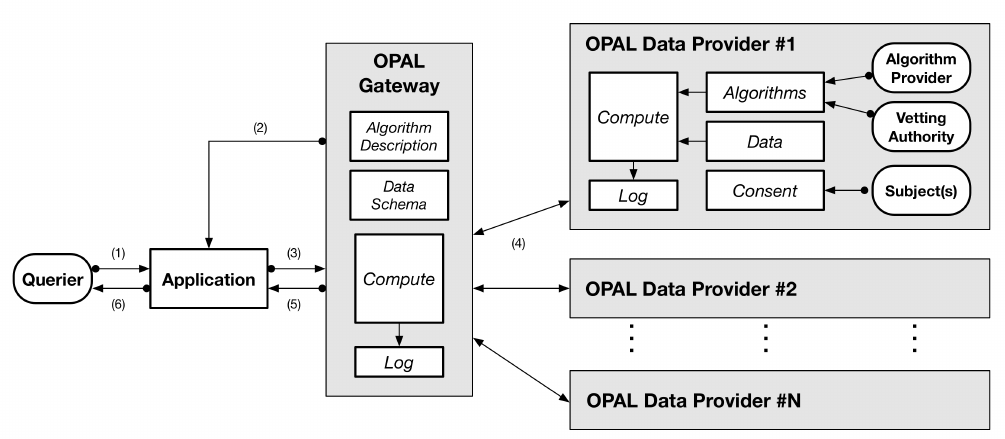
\includegraphics{images/png/OPAL-ecossytem.png}}
    \fonte{\citeonline{opal}}
    \label{fig:opal-ecossytem}
\end{figure}


\section{Standard for Machine Readable Personal Privacy Terms}

O Standard for Machine Readable Personal Privacy Terms é um padrão que será desenvolvido pelo grupo de trabalho \sigla{MRPTWG}{Machine Readable Privacy Terms Working Group} da IEEE. Seu objetivo é abordar a forma como os termos de privacidade pessoal são formulados e como esses termos podem ser lidos e aceitos por máquinas. Essa abordagem permitiria que dispositivos e sistemas em uma rede concordassem de maneira clara e precisa sobre a divulgação e o uso de informações. A relevância e o impacto desse padrão dependem, evidentemente, de sua implementação prática, o que o torna um tópico de interesse significativo para a evolução das políticas de privacidade digital. Portanto, merece ser mencionado aqui.

\section{Comparação entre propostas}

\begin{table}[h]
  \caption{Comparação entre Propostas}
  \label{tab:related}
  \resizebox{\textwidth}{!}{%
  \begin{tabular}{@{}lcccc@{}}
  \toprule
  \textbf{\color[HTML]{000000} Proposta}                                           & \textbf{\begin{tabular}[c]{@{}l@{}}Nível de\\ Atuação\end{tabular}}             & \textbf{\begin{tabular}[c]{@{}l@{}}Ambiente de\\ Execução\end{tabular}}           & \textbf{\begin{tabular}[c]{@{}l@{}}Dados\\ Compartilhados\end{tabular}}            & \textbf{\begin{tabular}[c]{@{}l@{}}Algoritmos\\ Verificados\end{tabular}}            \\ \midrule
  
  OPAL                                                                             & Modelo                                                                         & \begin{tabular}[c]{@{}c@{}}Provedor de \\ Dados\end{tabular}                       & sim                                                                                & sim                                                                                  \\ \midrule

  \begin{tabular}[c]{@{}l@{}}Machine Readable Personal Privacy Terms\end{tabular} & Padrão                                                                          & \begin{tabular}[c]{@{}c@{}}Sem informações\end{tabular}                            & Sem informações                                                                    & Sem informações                                                                      \\ \midrule 
  \begin{tabular}[c]{@{}l@{}}Novo Protocolo para \\ Modelo Fiduciário\end{tabular} & Protocolo                                                                      & \begin{tabular}[c]{@{}c@{}}SP, Fiduciário ou\\ ambos\end{tabular}                  & não                                                                                & não                                                                                  \\ \bottomrule
  \end{tabular}%
  }
  \fonte{O Autor}
  \end{table}
  

A \autoref{tab:related} oferece uma comparação entre as duas propostas em relação a diferentes aspectos. Na coluna intitulada \textbf{Nível de Atuação}, observa-se a primeira grande diferença entre as propostas. Enquanto a \acs{OPAL} é descrita como um "Modelo", o "Novo Protocolo para o Modelo Fiduciário" é classificado como um "Protocolo". Essa distinção é crucial, pois destaca o objetivo principal de cada solução proposta. Em geral, um modelo está primariamente preocupado em descrever um ecossistema de forma abstrata, enfatizando seus princípios e fundamentos, ao invés de se concentrar em como implementar o modelo de maneira prática. Por outro lado, um protocolo aprofundará a descrição oferecida por um modelo, visando facilitar sua implementação prática.

Em termos de \textbf{Ambiente de Execução}, o \acs{OPAL} opera exclusivamente no "Provedor de Dados", o que sugere uma mudança drástica em relação ao cenário atual. Por outro lado, o novo protocolo pode ser implementado no SP, no fiduciário ou em ambos, o que indica uma transição mais gradual para a execução de algoritmos em ambientes que oferecem maior confiança ao usuário. Na coluna \textbf{Dados Compartilhados}, o \acs{OPAL} possibilita o compartilhamento de dados, alinhando-se com práticas que promovem a colaboração. Em contraste, o novo protocolo não apresenta mecanismos específicos para o compartilhamento de dados. No entanto, o Modelo Fiduciário não impõe restrições a esse respeito, pois é viável que um fiduciário, com usuários de diferentes domínios, permita o compartilhamento de suas credenciais por meio de sua Política de Consentimento, visando adquirir novas análises sobre os dados.

Na coluna \textbf{Algoritmos Verificados}, o \acs{OPAL} também restringe seu escopo de atuação ao exigir, como princípio básico, a verificação de algoritmos. Essa exigência, por um lado, contribui para garantir a qualidade e a integridade das análises realizadas; por outro, pode atrasar o desenvolvimento de algoritmos mais atualizados e eficientes. Em contraste, o novo protocolo não incorpora nenhuma funcionalidade similar para a verificação de algoritmos, permitindo que o \acs{SP} apresente sua solução desejada, enquanto o fiduciário avalia se a proposta está de acordo com as definições de transparência e com as restrições impostas pelo seu beneficiário.




